\chapter{Characterising (Justus)}
\label{sec:Characterising}



\section{Allgemeines}
\label{sec:Unit}
Nachdem am ersten Labortag der Sensor mit Hilfe von SolidWorks designt und auf theoretischer Grundlage mit verschiedenen Simulationen berechnet wurde, musste am darauffolgenden Labortag eine Charakterisierung erfolgen. Aufgrund von Fertigungsabweichungen, die nie vermieden werden k�nnen, verhalten sich Sensoren immer unterschiedlich. Dies spiegelt sich unter Anderem in der Sensitivit�t, dem Offset oder auch in der Messgenauigkeit wider. Um den Abweichungen entgegenzuwirken, m�ssen bestimmte Eigenschaften des entsprechenden Sensors also zun�chst ermittelt werden.
Das IMT stellte jedem Laborteilnehmer einen vorgefertigten Sensor zur Verf�gung, der dem erstellten Design vom vorherigen Labortag entsprach. Lediglich bei der Betrachtung unter dem Mikroskop lie�en sich Differenzen feststellen. Der Unterschied zwischen den Drucksensoren ergab sich aus der Anordnung der jeweiligen Resistoren, die stellenweise in die Sensormembran eingearbeitet sind und der piezoresistiven Spannungsmessung dienen.
%INCLUDE SENSORBILDER UNTER MIKROSKOP
Abbildung 5.1 a) zeigt eine t-f�rmige Anordnung der Resistoren, Abbildung 5.1 b) eine longitudinale. Eine Festlegung, welche Anordnung f�r die gegebenen Anforderungen am besten geeignet sei, erfolgte durch �berlegung. %WARUM ??
\\
\begin{figure}[h]
    \subfigure[Messbr�cke mit t-f�rmiger Anordnung]{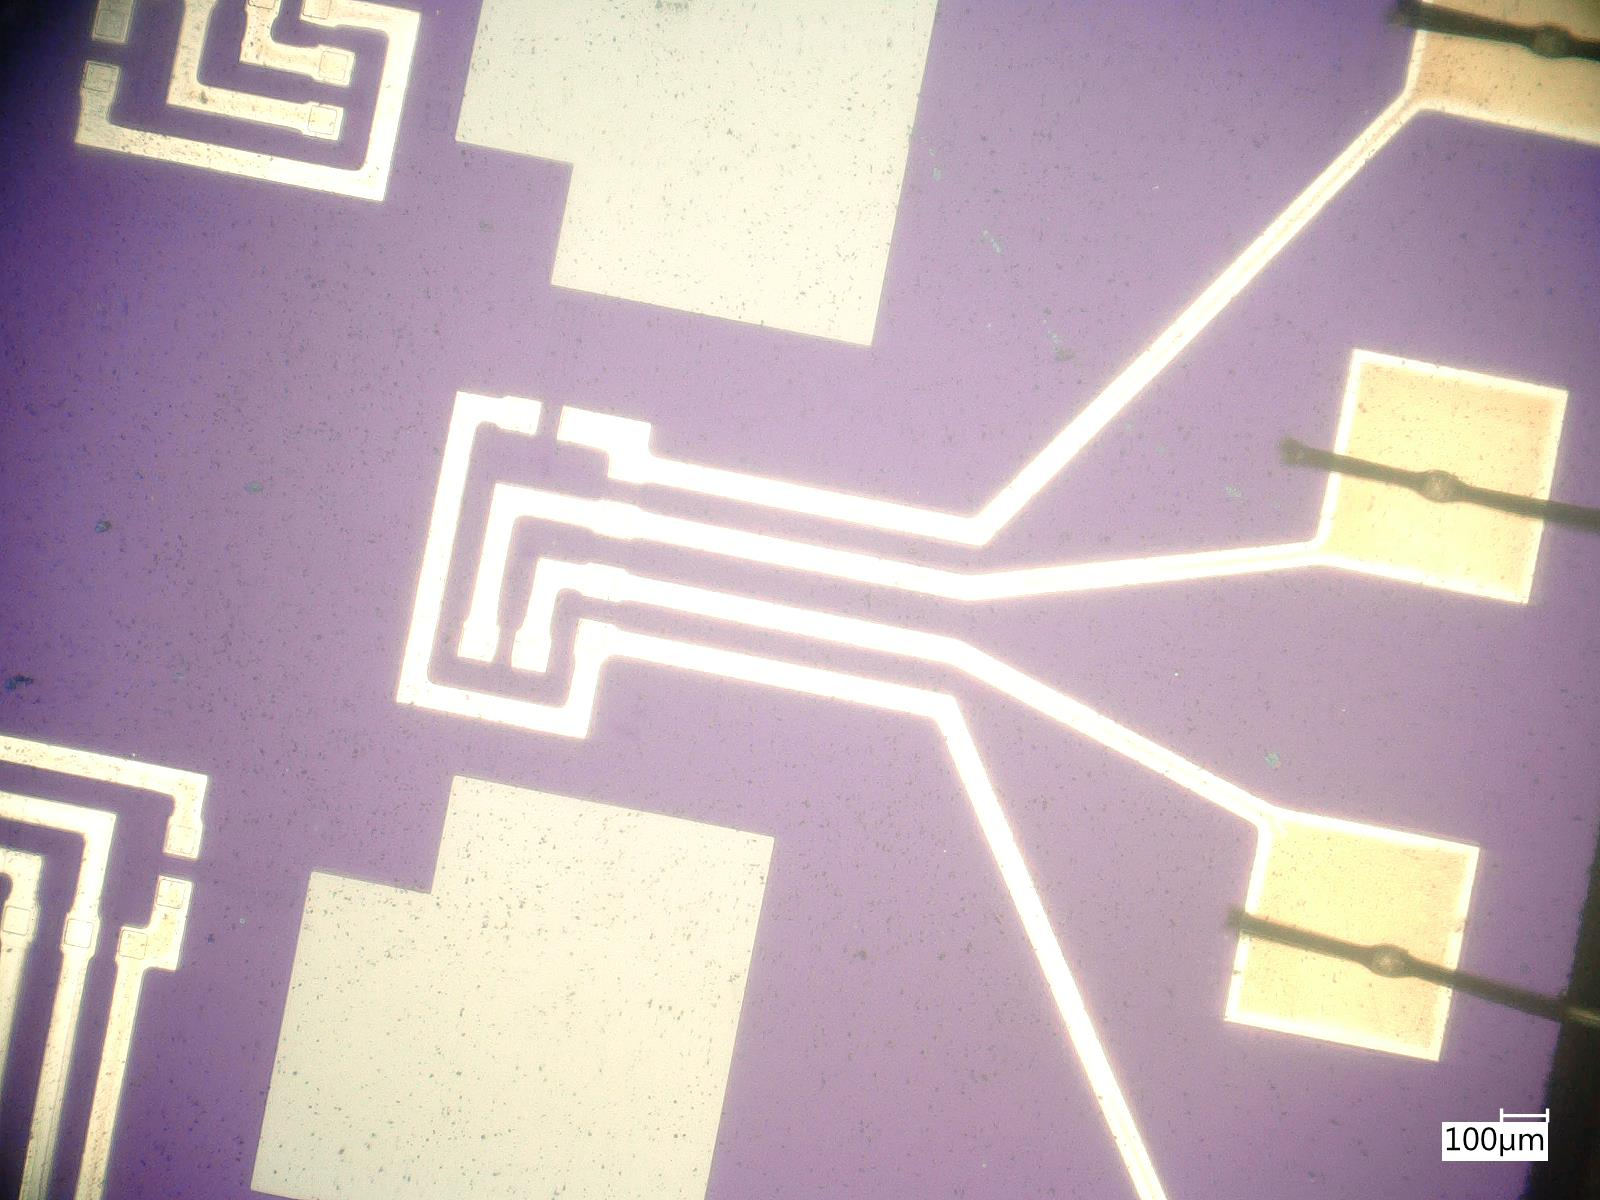
\includegraphics[width=0.49\textwidth]{figures/microscope_sensor/M_11_sensor.jpg}}
    \subfigure[Messbr�cke mit longitudinaler Anordnung]{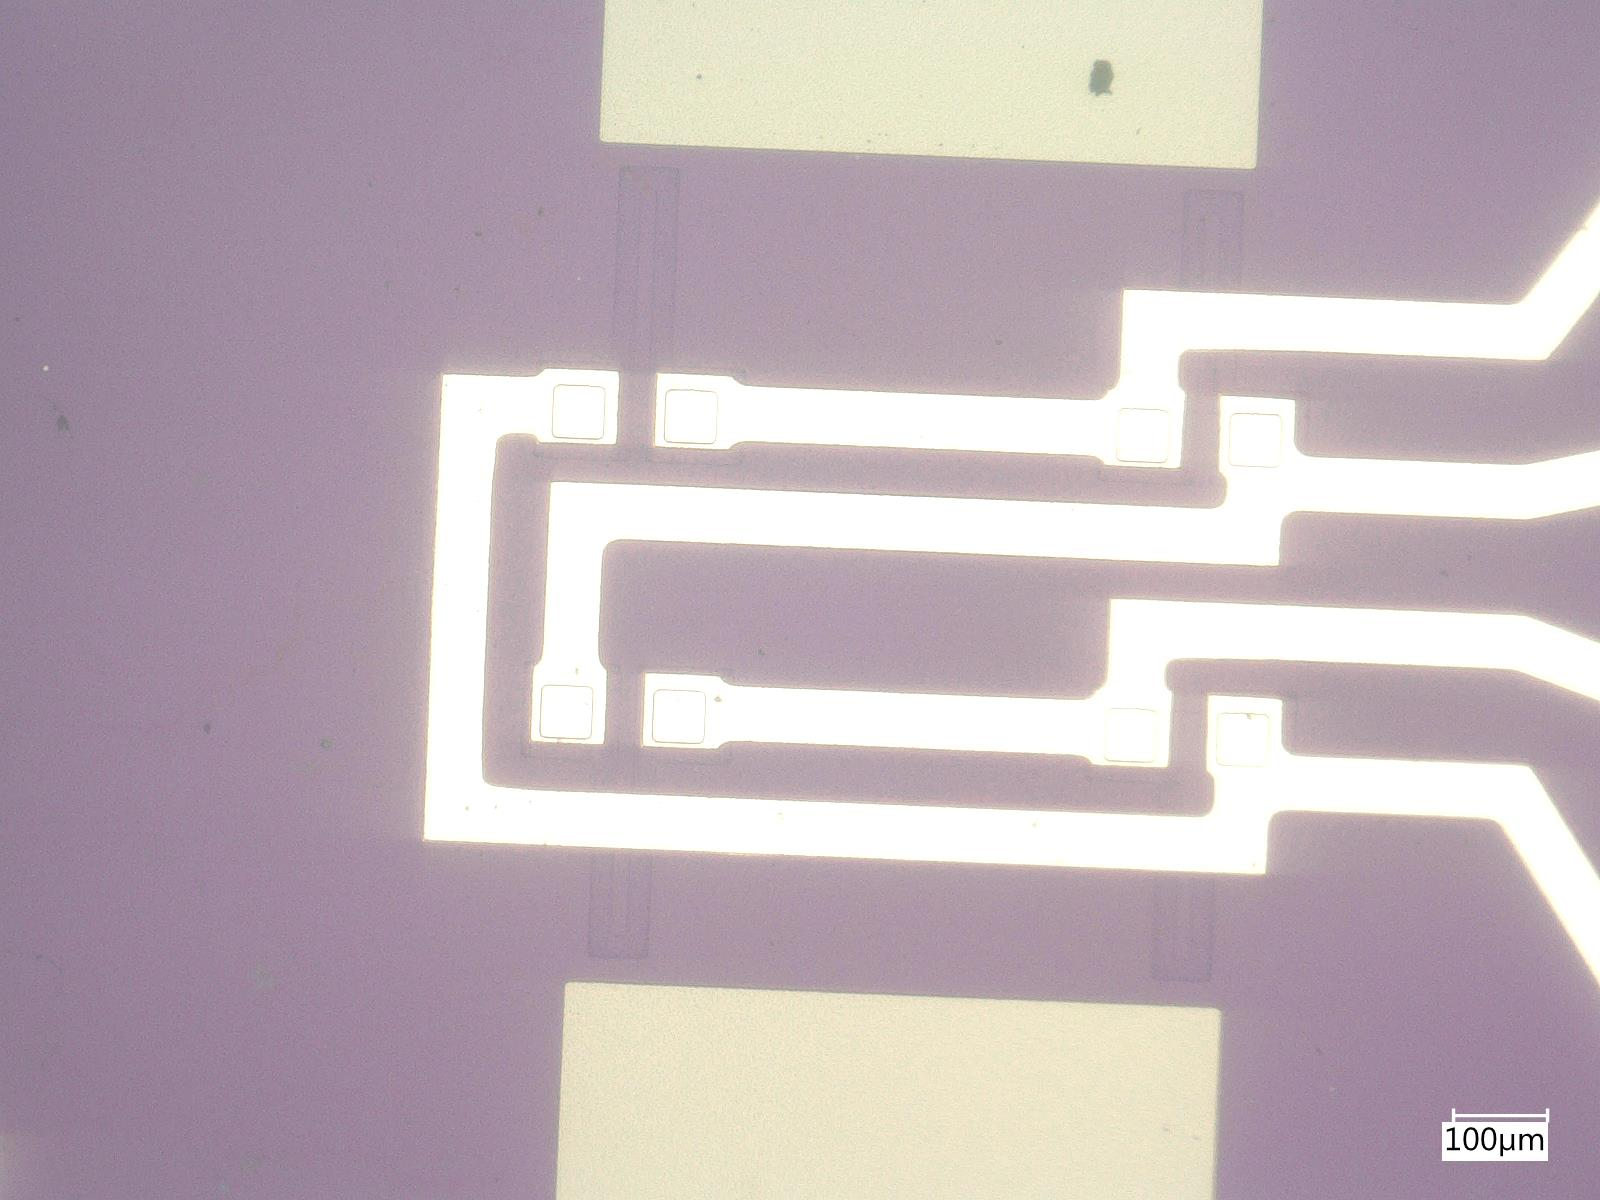
\includegraphics[width=0.49\textwidth]{figures/microscope_sensor/Justus_Sensor-13_200.jpg}}
\caption{Sensordesigns im �berblick}
\end{figure}\\

Anschlie�end begann die eigentliche Charakterisierung in Form eines Versuchs.
%Viele Einheiten lassen sich sch�ner darstellen mit dem "`Tag"' \verb|\unit[]{}| beziehungsweise \verb|\unitfrac[]{}{}|. Siehe den Vergleich: ohne 1~m oder mit \unit[1]{m} bzw. ohne 1~m/sec oder mit \unitfrac[1]{m}{sec}.

\section{Versuchsaufbau und -durchf�hrung}
\label{sec:Quelltext}
Der Sensor wurde auf eine Steckplatine mit entsprechenden Ein- und Ausg�ngen gesetzt. Die Versorgungsspannung von 1V wurde durch eine externe Spannungsquelle bewerkstelligt. Zur Messung der Ausgangsspannung stand ein Potentiometer zur Verf�gung, das ebenfalls mit der Steckplatine verbunden wurde. Bevor die Verbindungen angebracht wurden, mussten zun�chst die Leiterbahnen der Platine betrachtet werden, um Ein- und Ausg�nge nicht zu verwechseln. Der Druck wurde mit Hilfe eines Druckreglers aufgegeben, welcher den Gasdruck von Stickstoff exakt aufbringen konnte. Abbildung 5.2 zeigt den gesamten Versuchsaufbau.

\begin{figure}[h]
  \centering
  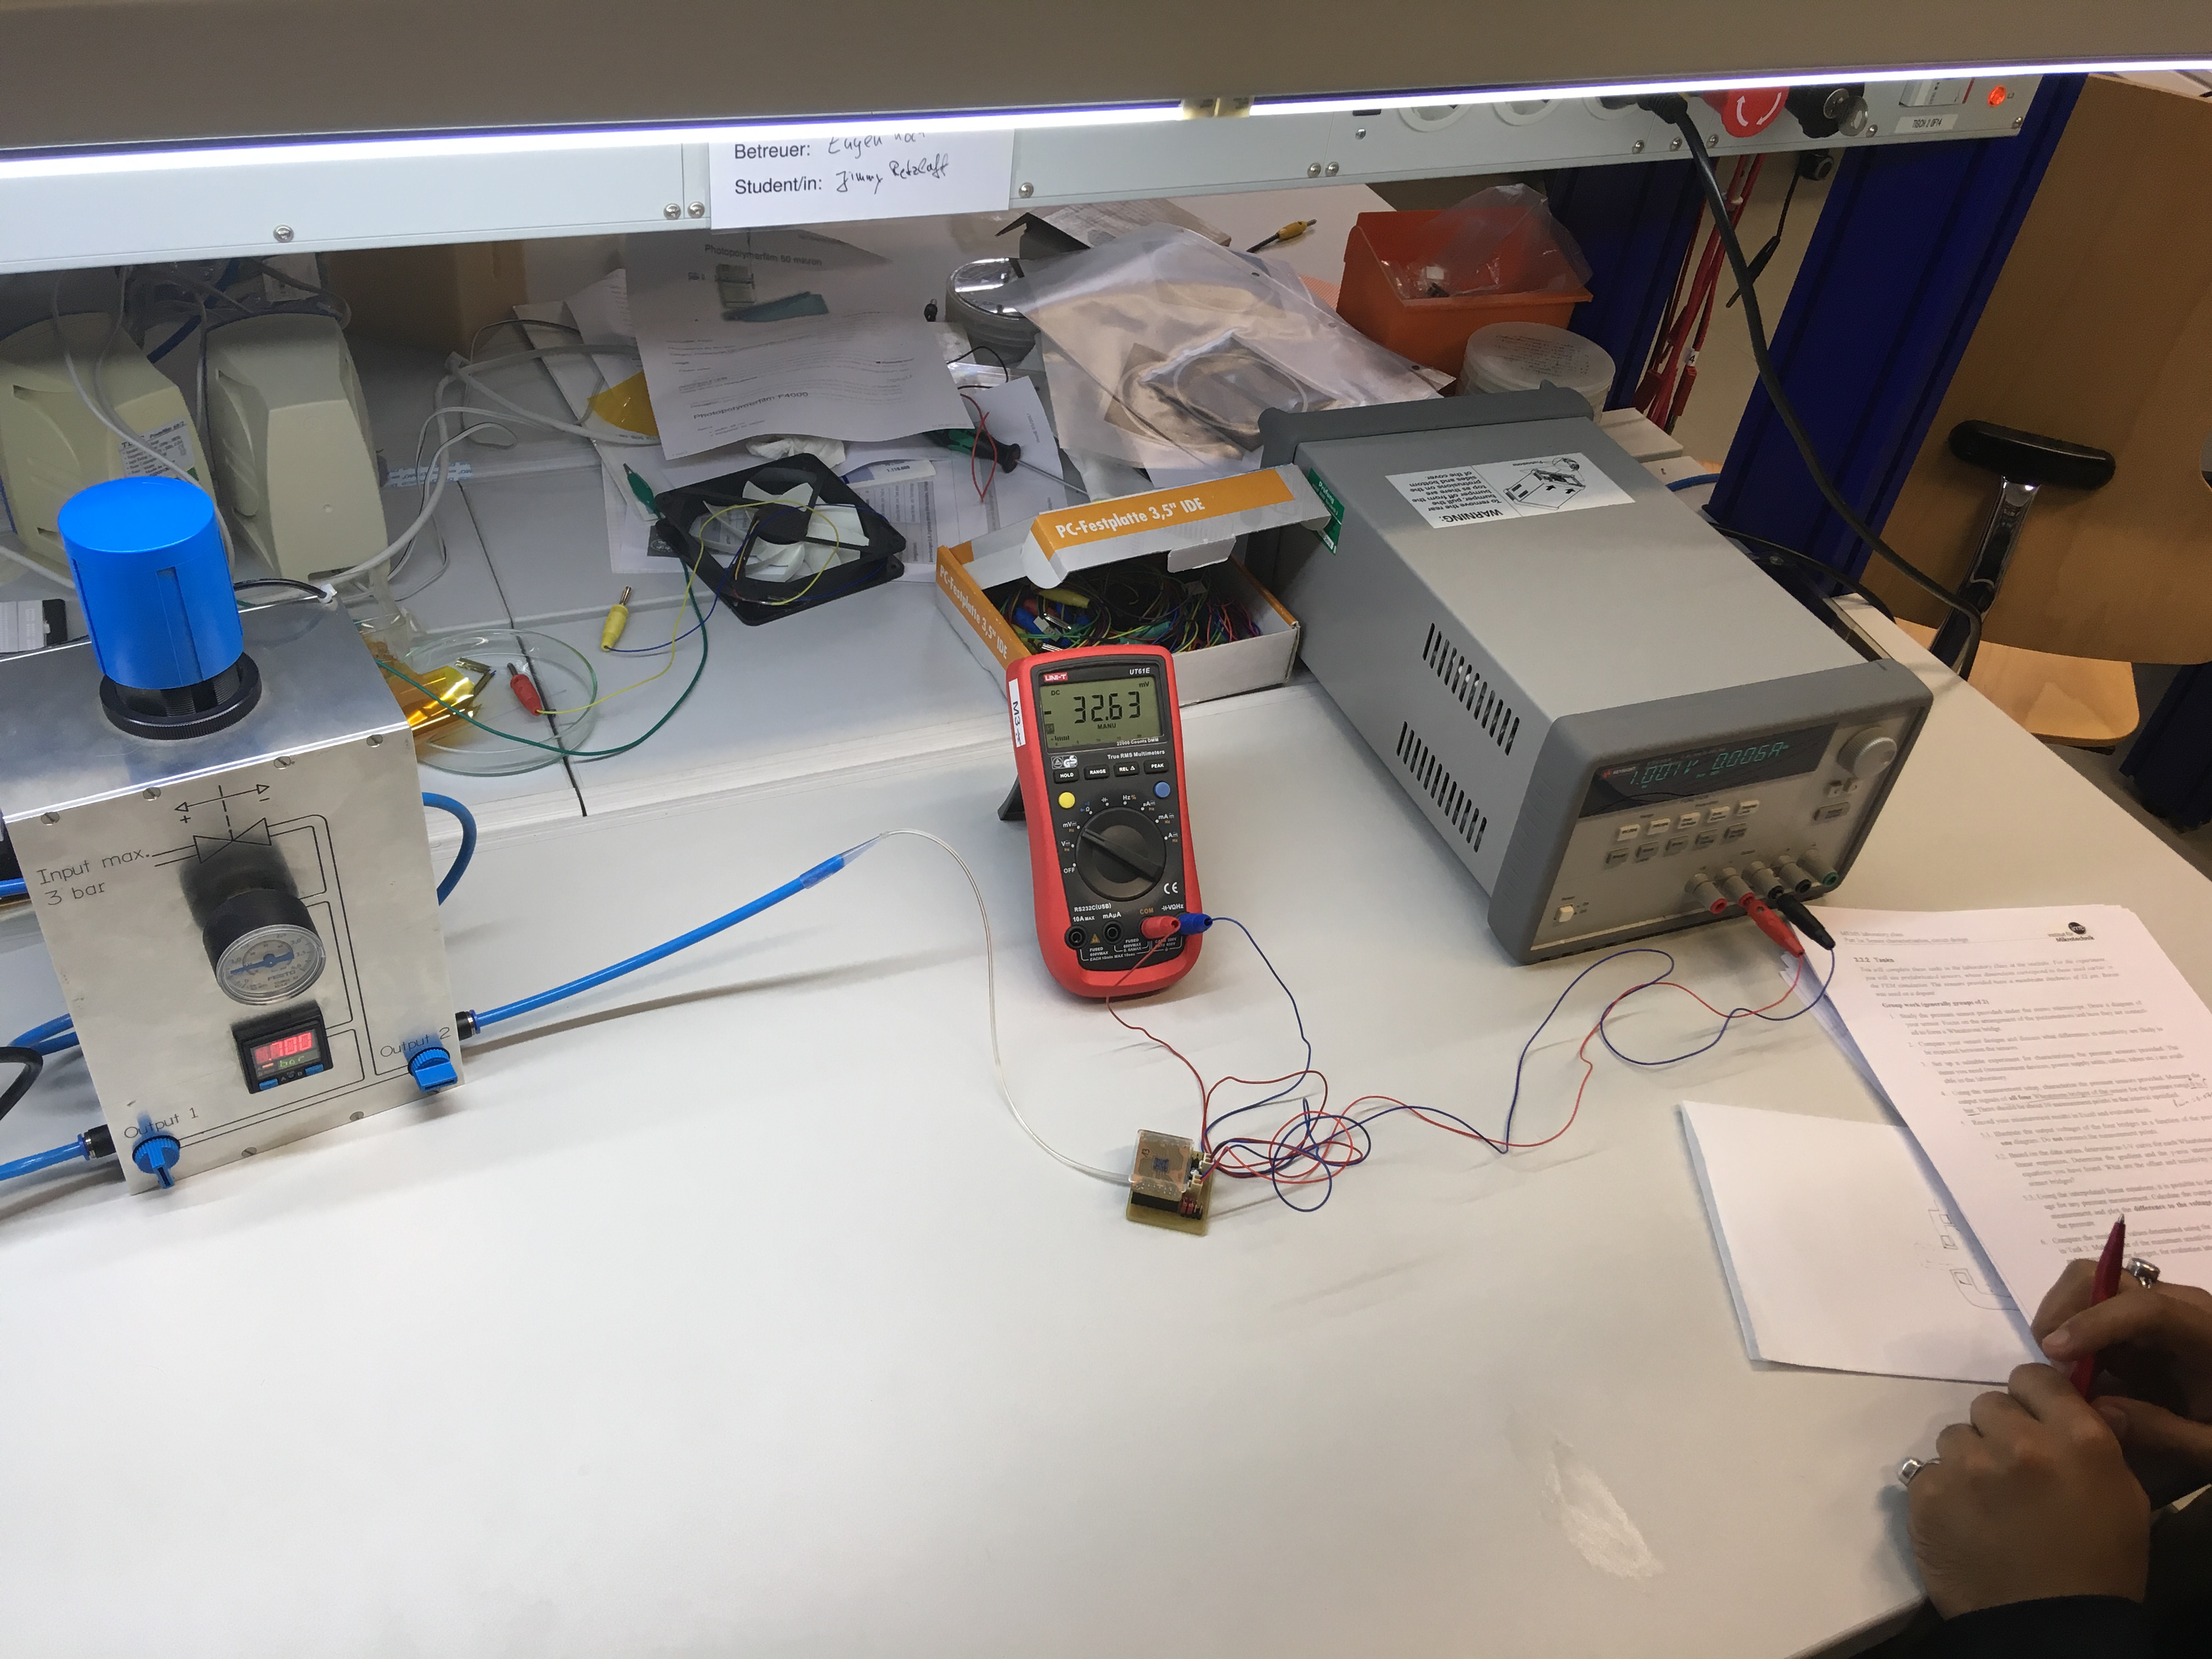
\includegraphics[width=0.7\textwidth]{figures/Versuchsaufbau1.jpg}
  \caption{Versuchsaufbau zur Charakterisierung}
  \label{fig:singlepicture}
\end{figure}

Da jede der vier zum Sensor geh�renden Wheatstone'schen Messbr�cken charakterisiert werden mussten, wurden entsprechende Jumper verwendet, mit denen die einzelnen Messbr�cken angesteuert werden konnten. Zu jeder Br�cke wurde die Ausgangsspannung f�r die Dr�cke 0bar, 0,2bar, 0,4bar, 0,6bar, 0,8bar und 1bar gemessen und festgehalten. Au�erdem wurde je eine Messung ohne Anschluss an die Druckversorgung durchgef�hrt, um einen Messwert unter atmosph�rischem Druck zu erhalten. 
Da eine folgende Aufgabe darin bestand, die gemessenen Werte mit denen einer anderen Laborgruppe zu vergleichen, wurde der Versuch noch mit einem weiteren Sensor durchgef�hrt. 
\section{Auswertung}
\label{sec:pictures}
Die gemessenen Werte wurden anschlie�end mit Hilfe von Microsoft Excel ausgewertet.


\begin{figure}[htbp]
  \centering
  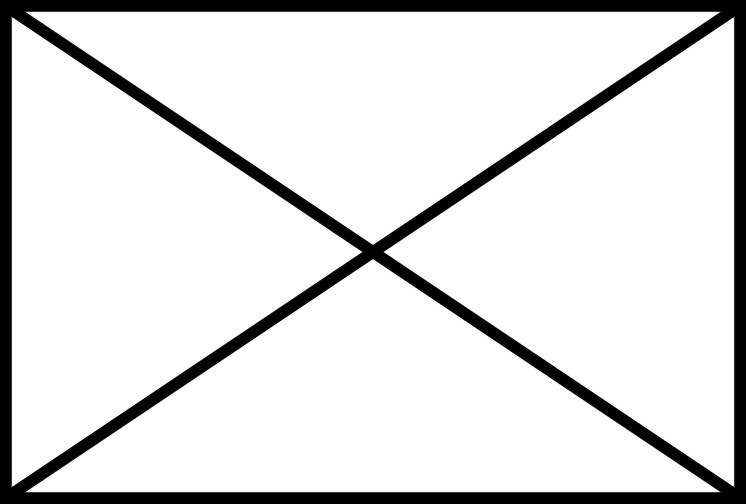
\includegraphics{figures/empty.jpg}
  \caption{Einzelne Abbildung}
  \label{fig:singlepicture}
\end{figure}




